% Created 2020-10-21 Wed 11:28
% Intended LaTeX compiler: lualatex
\documentclass[11pt]{article}
\usepackage{graphicx}
\usepackage{grffile}
\usepackage{longtable}
\usepackage{wrapfig}
\usepackage{rotating}
\usepackage[normalem]{ulem}
\usepackage{amsmath}
\usepackage{textcomp}
\usepackage{amssymb}
\usepackage{capt-of}
\usepackage{hyperref}
\usepackage{tabularx}
\usepackage{etoolbox}
\makeatletter
\def\dontdofcolorbox{\renewcommand\fcolorbox[4][]{##4}}
\AtBeginEnvironment{minted}{\dontdofcolorbox}
\makeatother
\usepackage[newfloat]{minted}
\usepackage{amsthm}
\theoremstyle{definition}
\newtheorem{definition}{Definition}[section]
\usepackage{unicode-math}
\usepackage{unicode}
\author{Mark Armstrong}
\date{Fall 2020}
\title{Bindings and scope\\\medskip
\large Principles of Programming Languages}
\hypersetup{
   pdfauthor={Mark Armstrong},
   pdftitle={Bindings and scope},
   pdfkeywords={},
   pdfsubject={Definition and tools for building formal languages. Introduction to semantics.},
   pdfcreator={Emacs 27.0.90 (Org mode 9.4)},
   pdflang={English},
   colorlinks,
   linkcolor=blue,
   citecolor=blue,
   urlcolor=blue
   }
\begin{document}

\maketitle

\section{Preamble}
\label{sec:org06ee6d7}
\subsection{Notable references}
\label{sec:org8b8c03a}
\begin{itemize}
\item Robert W. Sebesta, “Concepts of Programming Languages” (10th edition)
\begin{itemize}
\item Chapter 5, Names, Bindings, and Scopes
\end{itemize}
\end{itemize}

\subsection{{\bfseries\sffamily TODO} Table of contents}
\label{sec:orge870e59}
\begin{scriptsize}
\begin{itemize}
\item \hyperref[sec:org06ee6d7]{Preamble}
\end{itemize}
\end{scriptsize}

\section{Introduction}
\label{sec:org26d74ec}
This section introduces several concepts
relating to names and bindings of those names.

Of particular note is \emph{scope}, the “visibility” of names
throughout a program.

\subsection{What's a binding?}
\label{sec:orgfd4bfac}
A \emph{binding} is a general term that refers
to any association between an entity and an attribute.
\begin{itemize}
\item This is a very vague definition, which allows us to apply it
to a great many instances.
\end{itemize}

The \emph{entities} are “syntactic units” of the language.
\begin{itemize}
\item That is, some piece of the language syntax.
\end{itemize}

The \emph{attributes} may happen to also an entity of the language,
or may be a more “external” concept.

For instance,
\begin{itemize}
\item a variable (entity) will usually have a name (attribute)
\begin{itemize}
\item and often a type (attribute),
\end{itemize}
\item a type (entity) should have also have a name (attribute.)
\end{itemize}

In these notes, we primarily discuss bindings of \emph{types}, \emph{lifetimes} and \emph{scopes}.
Other bindings may come up later in the course.

\subsection{Uses of names}
\label{sec:orga5d15d9}
Many entities may be have names bound to them;
\begin{itemize}
\item variables, constants, parameters/arguments,
\item functions, methods, procedures, subroutines,
\item modules, packages, contexts, typeclasses, records, and
\item types,
\end{itemize}
to name a few.

\subsection{Persistance of names}
\label{sec:org5c0fe15}
Take note!
\begin{itemize}
\item Some namings are “global”; they persist for “all time and space”.
\begin{itemize}
\item Such as the namings of builtin language methods,
\begin{itemize}
\item (assuming the language does not allow their names to be reused
or shadowed.)
\end{itemize}
\end{itemize}
\item But many namings are temporary!
\begin{itemize}
\item And one instance of a name may shadow another.
\begin{itemize}
\item (Such as when you declare a local variable/argument
with the same name as one already in scope.)
\end{itemize}
\end{itemize}
\end{itemize}

\subsection{A note about time and space}
\label{sec:org7eb2818}
Throughout these notes, we will discuss \emph{when} and \emph{where} bindings
are in effect.

These discussions of “time” and “space” are relative to the program.
\begin{itemize}
\item Our notion of “\emph{time}” is in terms of the program's runtime.
\begin{itemize}
\item Or occasionally, its design time.
\end{itemize}
\item Our notion of “\emph{space}” is in terms of the program's \emph{text}.
\end{itemize}

\subsection{Static and dynamic bindings (or “checking of bindings”)}
\label{sec:org5d50d34}
Bindings which are decided (or known) \emph{before} runtime
are called \emph{static}.

Conversely, bindings which are not decided (or known) until \emph{during} runtime
are called \emph{dynamic}.

We say “or known” because some bindings, such as the types of values,
are not so much “decided” as “discovered”.
\begin{itemize}
\item All values have a type, whether or not that type is checked
statically or dynamically.
\end{itemize}

\section{Type checking and polymorphism}
\label{sec:org051166b}
Type checking is the process of determining
the binding between a name of an entity and a type.
\begin{itemize}
\item Usually, only variables, arguments, functions and similar entities
have types.
\begin{itemize}
\item There is at least one exception to this;
sometimes, types may have a type!
\end{itemize}
\item We will discuss types in more detail in the next section.
\end{itemize}

\subsection{“Dynamically checked” instead of “dynamically typed”}
\label{sec:orgbe6df73}
As with many bindings, languages can be categorised as
being either \emph{statically} or \emph{dynamically} typed.

In “Types and Programming Languages”, though, Pierce argues
that the term “dynamically typed language” is a misnomer.
\begin{itemize}
\item It would be better to say “dynamically (type) checked”.
\item All values have a type, even before type checking.
\end{itemize}

\subsection{Static and dynamic type checking}
\label{sec:orgf2b1436}
It's somewhat natural for interpreted languages to be dynamically typed,
and compiled languages to be statically typed.
\begin{itemize}
\item The process of type checking is an upfront cost.
\begin{itemize}
\item Compilation is a natural time to carry out that costly process.
\end{itemize}
\item Consider the (primarily) interpreted “scripting” languages;
Python, Ruby, Javascript, Lua, Perl, PHP, etc.
\item But it's far from universally true that interpreters use
dynamic typing!
\begin{itemize}
\item Haskell has an interpreter, and is definitely
statically typed.
\end{itemize}
\end{itemize}

\subsection{Polymorphism}
\label{sec:org6e48263}
Assigning each value in a program a single type, and then
enforcing type correctness (preventint type clashes)
introduces a (solveable) problem; it prohibits code reuse!
\begin{itemize}
\item Subroutines can only be used on a particular type of arguments.
\end{itemize}

Subtyping and polymorphism provide solutions to this.
\begin{itemize}
\item With \emph{subtyping}, there is a sub/super relation between types.
\begin{itemize}
\item One classic examples involves a type of “shapes”, which has
a subtype “polygon”, which in turn has subtypes “triangle”
and “rectangle”, etc.
\item Subtypes closely resemble the notion of \emph{subsets}.
\item Values of a subtype can be used anywhere
a value of their supertype is expected.
\item Sub-\emph{classing} is one instance of subtyping.
\begin{itemize}
\item And is usually just called subtyping.
\end{itemize}
\item Subranges and, sometimes, enumeration types are other examples.
\end{itemize}
\item With \emph{polymorphism}, a subroutine can have several types.
\end{itemize}

\subsection{Ad hoc polymorphism (overloading)}
\label{sec:org5734ee9}
One notion of polymorphism is \emph{ad hoc} polymorphism,
also called \emph{overloading}.
\begin{itemize}
\item With overloading, subroutine names
can be reused as long as the types of arguments
differ (in some specified way.)
\item The downside is the programmer must define
the “same” subroutine many times; once for each type.
\end{itemize}

Here is an example of ad hoc polymorphism in Scala.
\begin{minted}[breaklines=true]{scala}
def sum(a: Int, b: Int): Int = a + b
def sum(a: Boolean, b: Boolean): Boolean = a || b
\end{minted}

\subsection{Parametric polymorphism}
\label{sec:orgace2543}
With parametric polymorphism, subroutines have a
\emph{most general} type, based on the \emph{shape} or \emph{form} of their arguments.
\begin{itemize}
\item This involves the use of \emph{type variables}.
\item The subroutines behaviour can only be based on the form,
not the specific types.
\item This is commonly used in functional languages.
\begin{itemize}
\item Several object-oriented languages have \emph{generics}, which are
essentially the same concept.
\end{itemize}
\end{itemize}

Here is an example of parametric polymorphism in Scala.
\begin{minted}[breaklines=true]{scala}
def swap[A](p : Tuple2[A,A]): Tuple2[A,A] = p match {
  case (p1, p2) => (p2, p1)
}
\end{minted}

\subsection{Duck typing}
\label{sec:org88d7e6a}
More formally called \emph{row polymorphism}.
\begin{itemize}
\item Duck typing does not actually check the types of values.
\item It is used when calling a method on a value;
the only check is that that method is defined for that value.
\item “If it walks like a duck, and quacks like a duck, it's a duck!”
\end{itemize}

Here is an example of duck typing in Ruby.
\begin{minted}[breaklines=true]{ruby}
class Thing1
  def initialize(v,w); @v = v; @w = w end
  def do_the_thing() "I'll implement this later." end
end

class Thing2
  def initialize(v,w); @v = v; @w = w end
  def do_the_thing() @v + @w end
end
  
def doit(x) x.do_the_thing end

x = Thing1.new(1,2)
y = Thing2.new(1,2)

puts doit(x) # Outputs a string
puts doit(y) # Outputs an integer
\end{minted}

\section{Lifetime}
\label{sec:org0c9fc0b}
The \emph{lifetime} of an entity is the portion of the runtime
(not the code) during which that entity has allocated memory.

To discuss lifetimes, we first need to discuss
the layout of memory and the process of memory allocation.

\subsection{The data segment, stack, and heap}
\label{sec:orgcd5d82c}
In the context of running a program (or a thread of a program):
\begin{itemize}
\item The \emph{data segment} is a portion of memory used to store the
program itself and static/global variables.
\item The \emph{stack} is an organised portion of memory allocated for the program.
\begin{itemize}
\item Blocks at the “top” of the stack are reserved when entering
a scope.
\begin{itemize}
\item These blocks are called \emph{stack frames}.
\end{itemize}
\item Stack frames are \emph{popped off} the stack when leaving the unit of code.
\end{itemize}
\item The \emph{heap} is an unorganised portion of memory allocated for the program.
\begin{itemize}
\item Allocation/deallocation may be independent of units of code.
\item Disorganisation can lead to inefficiency and other problems.
\begin{itemize}
\item Cache misses, page faults, etc.
\item Running out of memory or appropriately sized continguous blocks.
\item Garbage, dangling references, etc.
\end{itemize}
\end{itemize}
\end{itemize}

\subsection{Picturing memory}
\label{sec:orgcf7f7c0}
\begin{center}
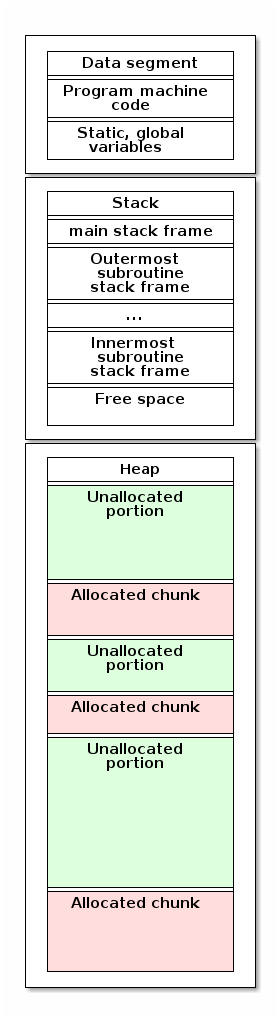
\includegraphics[width=\textwidth]{media/data-segment-stack-heap.png}
\end{center}

\subsection{Kinds of memory allocation}
\label{sec:org145c219}
We can distinguish four kinds of memory allocation;
\begin{itemize}
\item static,
\item stack dynamic,
\item implicit heap dynamic, and
\item explicit heap dynamic.
\end{itemize}

\subsection{Static and stack dynamic allocation}
\label{sec:org34df112}
\begin{itemize}
\item Static
\begin{itemize}
\item Allocation is done \emph{before runtime} (static), in the data segment.
\begin{itemize}
\item At load time, when the program is loaded into memory.
(Not compile time.)
\end{itemize}
\end{itemize}
\item Stack dynamic
\begin{itemize}
\item Allocation is dynamic, automatic, and on the stack.
\item Amount of memory needed must be known when entering their scope.
\item This is “the usual method” in most imperative languages.
\end{itemize}
\end{itemize}

\subsection{Implicit and explicit heap dynamic allocation}
\label{sec:org9b41642}
\begin{itemize}
\item Implicit heap dynamic
\begin{itemize}
\item Allocation is dynamic, automatic, and on the heap.
\item Memory is simply allocated when the variable is assigned;
the programmer does not need to “do anything”.
\end{itemize}
\item Explicit heap dynamic
\begin{itemize}
\item Allocation is dynamic, \emph{manual}, and on the heap.
\item The programmer must use a command to allocate memory
\emph{before} assignments can be made.
\begin{itemize}
\item E.g., \texttt{malloc} or \texttt{new}.
\end{itemize}
\item In fact these blocks of memory can be considered
\emph{nameless variables}; we need other,
\emph{reference} variables to \emph{point} to their address.
\end{itemize}
\end{itemize}

\subsection{Exercise: Memory allocation methods}
\label{sec:orgad1b70d}
Investigate:
\begin{itemize}
\item Which of the five kinds of memory allocation are available in
Scala and in Ruby.
\item How each kind of memory allocation is denoted.
\end{itemize}

\subsection{The lifetime}
\label{sec:org3779266}
To repeat,
the \emph{lifetime} of an entity is the portion of the runtime
(not the code) during which that entity has allocated memory.
\begin{itemize}
\item There may be several \emph{instances} of a single variable in the code,
each with its own lifetime.
\item The lifetime of a variable depends upon the memory allocation
strategy used for it.
\begin{itemize}
\item \textbf{Static}: lifetime is the whole of runtime.
\item \textbf{Stack dynamic}: lifetime is the portion of runtime between
when the scope containing the variable is entered
and when control returns to the invoker of that scope.
\begin{itemize}
\item In the case of functions/procedures, local variables
end their lifetime when the function/procedure returns.
\item Note that a variable may go out of scope, but still be alive.
\end{itemize}
\item \textbf{Implicit heap-dynamic}: lifetime begins when assigned.
The end of lifetime depends upon garbage collection.
\item \textbf{Explicit heap-dynamic}: lifetime begins when the allocation
command is used. The end of lifetime may be
\begin{itemize}
\item when the programmer issues a deallocation command, or
\item depend upon garbage collection.
\end{itemize}
\end{itemize}
\end{itemize}

\subsection{Garbage collection}
\label{sec:org2a32e22}
\emph{Garbage} is allocated memory which is no longer accessible.

\emph{Garbage collection} is the process of deallocating garbage.
\begin{itemize}
\item A complex activity.
\begin{itemize}
\item We will discuss the basics here, and then likely not
touch on it again.
\item Has a large influence on the efficiency of
compiled/interpreted code.
\end{itemize}
\item There are two main categories of garbage collection algorithms;
\begin{itemize}
\item tracing,
\begin{itemize}
\item which includes the “mark \& sweep” algorithm, and
\end{itemize}
\item reference counting.
\end{itemize}
\item Additionally, language implementations may include compile time
“escape analysis”.
\begin{itemize}
\item Memory may be allocated off the stack instead of the heap
\emph{if} no references to the variable are available outside its scope
(if it doesn't “escape”.)
\end{itemize}
\end{itemize}

\subsubsection{Tracing garbage collection (mark \& sweep)}
\label{sec:org9152e54}
\begin{itemize}
\item Usually triggered when a certain memory threshold is reached.
\item Starting from some set of base references
(usually those in the stack and data segment),
“trace” references, somehow marking those that are reachable.
\begin{itemize}
\item Starting from the set of base references,
“determine the transitive closure of reachability”.
\end{itemize}
\item Once done, free any memory that is not marked.
\item “Naive” mark \& sweep:
\begin{itemize}
\item Each object in memory has a bitflag for this “marking”,
kept clear except during garbage collection.
\item When activated, traverse all reachable memory,
“marking” what's reached, then “sweep” away all unmarked memory
(and reset the flags of marked memory.)
\begin{itemize}
\item With this naive approach, we have to pause the program to do this;
\item better methods do not require pausing.
\end{itemize}
\end{itemize}
\end{itemize}

\subsubsection{Reference counting garbage collection}
\label{sec:org49057c0}
\begin{itemize}
\item An “eager” approach.
\item As the program runs, keep a count of the number of references
to every object in memory.
\begin{itemize}
\item So we must perform some tallying on every assignment!
\end{itemize}
\item When the number of references reaches zero, we can free the memory
for that object.
\item This approach needs to account for cycles, though!
\begin{itemize}
\item Every object in a cyclic (portion of a) data structure
will always have at least one pointer to it,
even if the structure as a whole is unreachable.
\item This necessity increases the overhead.
\end{itemize}
\end{itemize}

\subsection{Dangling/wild references}
\label{sec:orgb5e28f7}
Garbage is not the only problem that can occur with
references to memory.

A \emph{dangling} or \emph{wild} reference is a reference to memory
which has already been freed.
\begin{itemize}
\item Presumably, by a programmer's action.
\item After being freed, memory may be left as is until it
is allocated again, or may be wiped in some way.
\begin{itemize}
\item Accessing memory that is no longer reserved
usually leads to undefined behaviour.
\end{itemize}
\end{itemize}

We will discuss methods of preventing use of wild/dangling references
when we discuss reference types later in the course.

\section{Scope}
\label{sec:org05d4793}
A \emph{scope} (singular) is a portion of the program to which the visibility
of entities may be limited.
\begin{itemize}
\item This is a design decision: what constructs introduce scopes?
\begin{itemize}
\item Almost certainly subroutines do.
\item Do conditional branches? Loop bodies?
\end{itemize}
\item As a general term, within this section we say \emph{block} for a construct which
introduces a scope.
\begin{itemize}
\item Outside of this section, we have used and will continue to use the
singular \emph{scope} for this, but here that will conflict with
the adjective scope we are about to define.
\end{itemize}
\end{itemize}

\subsection{Static scoping}
\label{sec:orgd2c250c}
The \emph{scope} (adjective) of an entity is the portion of the program
in which it is “visible”.
\begin{itemize}
\item Usually scope is statically determined.
\begin{itemize}
\item It is usually the block in which it is defined,
and all subblocks of that block,
\begin{itemize}
\item unless it is shadowed by another entity of the same name.
\end{itemize}
\end{itemize}
\item Static scoping is so pervasive, you have likely
never come across a language where scope works differently,
outside of differences in what constructs introduce scope.
\end{itemize}

\subsection{Dynamic scoping}
\label{sec:orgae206ae}
With dynamic scoping, the scope of entities depends upon the
    “execution trace”, i.e., the “path” through the program.
\begin{itemize}
\item Dynamic scoping is rarely used.
\begin{itemize}
\item The detriments strongly outweigh the benefits in most cases.
\item The one major benefit is relief from having to pass arguments;
\end{itemize}
\end{itemize}

\subsection{Exercise: On dynamic scoping}
\label{sec:org2c12adf}
\begin{itemize}
\item Historically, Lisps (languages directly descended from Lisp)
were dynamically scoped.
\item Presently, the only widely used Lisp which uses dynamic scoping
by default is Emacs Lisp (eLisp.)
\end{itemize}

Try out this snippet of Emacs lisp code,
either in Emacs (if you have it) or using an
\href{https://repl.it/languages/elisp}{online REPL}.
\begin{minted}[breaklines=true]{common-lisp}
(let ((x 2) (y 5)) ; "global" variables x and y
  (progn
    (defun mult-x-y ()
      (* x y)) ; returns x * y

    (defun A ()
      (let ((x 3)) ; local variable x
        (mult-x-y)))

    (defun B ()
      (let ((y 10)) ; local variable y
        (A)))

    (message "mult-x-y returns %d, A returns %d and B returns %d"
      (mult-x-y) (A) (B))))
\end{minted}

\begin{enumerate}
\item Ensure you understand the results.
\item Using this understanding, formulate some advantages and disadvantages
of dynamic scoping.
\end{enumerate}

\subsection{Exercise: Entities which introduce scope}
\label{sec:orgd21fcd2}
In a few different programming languages, investigate whether
condition branches and loop bodies introduce scopes.

I.e., test out code such as
\begin{minted}[breaklines=true]{text}
if B then
  int x = 0
endif

y = x   % Is x still in scope?
\end{minted}

Specifically, investigate languages which have \emph{iterating loops},
(usually called \texttt{for} loops.) What is the scope of an iterator
for such loops?
\end{document}
